% arara: pdflatex: { draft: yes, shell: yes, options: [--output-directory=build] }

%! arara: makeglossaries: { options: [ '-d', 'build' ] }
%! arara: --> if changed (toFile('build/report.glo')) || missing (toFile('build/report.gls'))

% arara: pdflatex: { shell: yes, synctex: yes, options: [--output-directory=build] }

\documentclass{article}

\usepackage{settings/set-color}
\usepackage{settings/set-geometry}
\usepackage{settings/set-lists}
\usepackage{settings/set-graphics}
\usepackage{settings/set-tables}
\usepackage{settings/set-spacing}
\usepackage{settings/set-code}
\usepackage{settings/set-plots}

\begin{document}

\title{Introduction to Parallel Computing\\
    Homework 1: Implicit parallelism techniques and performance models.\\
    \textbf{Results report}
}
\author{Lorenzo Fasol, 18244, lorenzo.fasol@studenti.unitn.it}
\date{October 2023}
\maketitle

\section{Array addition and vectorization}
In the first section of the Homework, both \textit{Task1} and \textit{Task2} involve the element-wise addition of two arrays, defined as A and B. This operation is executed through the implementation of two distinct routines, denoted as \texttt{routine1()} and \texttt{routine1()}, respectively. The result of this addition is stored in another array, denoted as C, of the same size as arrays A and B.\\
%inserisci che le due rotuine sono uguali quindi la differenza è in compilazione
Given the necessity for Task 2 to incorporate implicit parallelism techniques, it's crucial to underscore that the actual code implementation for both tasks remains constant. While the code structure remains unaltered, the essential distinction emerges in how the compiler handles and optimizes the code.\\
\textit{Task1} can be seamlessly compiled to yield a sequential program, with no additional requirements. In contrast, \textit{Task2} demands the incorporation of specific compilation flags designed to harness implicit parallelism techniques. These flags are essential in the compilation process, enabling the code to exploit parallelism and optimize performance.\\
The compiler used, \texttt{GNU C++ compiler (G++)} in this specific case, offers a range of flag combinations for optimizing code. Following extensive experimentation to determine the most effective combination of these flags that leads to an optimal result, I have arrived at the following conclusions. Two potential solutions have emerged, yet I favor the second option due to its higher level of specificity and detail.\\\\
The solutions are the following:
\begin{itemize}
  \item \texttt{gcc -O3 hw1\_pt1.cpp -o hw1\_pt1.out}\\
  This only flag enable the utilization of a set of optimization like for example function in-lining and instruction scheduling that are not specific for parallelism but can be beneficial to achieve better performance.
  \item \texttt{gcc -O2 -ftree-vectorize -funroll-loops -fprefetch-loop-arrays -march=native hw1\_pt1.cpp -o hw1\_pt1.out}\\\\
  Flags explanation:
    \begin{itemize}
        \item[] \texttt{-O2}: applies a range of sophisticated optimization techniques aims to reduce the runtime execution time of the compiled program, thereby enhancing its efficiency and speed. 
        This optimization level strikes a balance, providing improved program efficiency without delving into more aggressive optimization levels, such as \texttt{-O3}.
        \item[] \texttt{-ftree-vectorize}: enable tree vectorization, which empowers the compiler to intelligently reconfigure loops. This optimization significantly enhance parallelism by enabling the simultaneous processing of multiple data elements within a single instruction.
        \item[] \texttt{-funroll-loops}: instructs the compiler to unroll loops. The compiler generates several duplicated instances of the loop body with the objective of mitigating the overhead associated with loops and to improve instruction-level parallelism.
        \item[] \texttt{-fprefetch-loop-arrays}: prompt the compiler to incorporate prefetching instructions within the generated code. Prefetching is a technique that aims to pre-load data into the cache before its actual demand, effectively mitigating data access latencies and enhancing parallelism.
        \item[] \texttt{-march=native}: used to optimize code for the specific microarchitecture of the host machine. Empowers the compiler to generate instructions that are finely tuned for the processor executing the code, maximizing performance. However, it ties the compiled code to the host machine's architecture.
    \end{itemize}
\end{itemize}
To conduct the tests, the default version of the program was employed, where three tests are performed for each array size within the range of $2^4$ to $2^{22}$. However, the C++ script can be executed with a user-defined array size by using a specific flag along with the corresponding argument. The test results have been stored in a \texttt{.CSV} file for the subsequent analysis. 

\subsection*{Results analysis}
ciao\\
ciao\\
ciao\\
ciao\\
ciao\\
ciao\\
ciao\\
%decidi quali risultati tenere se quelli del cluster o del fisso
AMD Ryzen\textsuperscript{\texttrademark} 2600x at 4.2GHz and 16GB of RAM.

\begin{figure}[htbp]
    \centering
    \captionsetup{
        type=plot,
        belowskip=10pt,
    }
    \caption{Loop execution times by array size}
    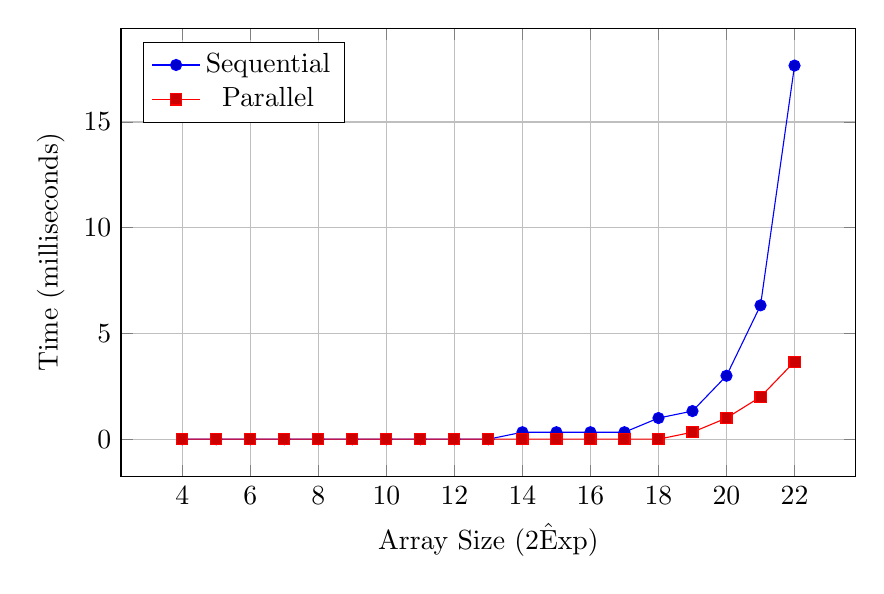
\begin{tikzpicture}
        \begin{axis}[
            width=0.9\textwidth,
            height=0.6\textwidth,
            xlabel={Array Size (2\^ Exp)},
            ylabel={Time (milliseconds)},
            legend pos=north west,
            grid=major,
        ]

        \addplot table [x=Exp, y=Average] {
            Exp Average
            4	0
            5	0
            6	0
            7	0
            8	0
            9	0
            10	0
            11	0
            12	0
            13	0
            14	0.33
            15	0.33
            16	0.33
            17	0.33
            18	1.00
            19	1.33
            20	3.00
            21	6.33
            22	17.67
        };

        \addplot table [x=Exp, y=Average] {
            Exp Average
            4	0
            5   0
            6   0
            7   0
            8   0
            9   0
            10  0
            11  0
            12  0
            13  0
            14  0
            15  0
            16  0
            17  0
            18  0
            19  0.33
            20  1.00
            21  2.00
            22  3.67
        };
        \legend{Sequential, Parallel}

        \end{axis}
    \end{tikzpicture}
\end{figure}

\section{Matrix copy via block reverse ordering}
In the second section of the homework, like the preceding section, both \textit{Task1} and \textit{Task2} entail the execution of identical actions.%
In this instance, the primary emphasis remains directed toward the compilation flags employed during the compilation process. The compilation commands and their associated flags remain unchanged from those utilized in previous instances but applied to the code files specific to this part.\\
In this scenario, the program operates on a matrix, defined as M, with a size denoted as n, which is simplified for clarity to be a power of two. %
The matrix is divided into blocks, each with a size of b.\\
The primary task involves performing a specific action: copying each block, along with its associated content, in the reverse order, while assuming a row-major ordering (with the internal order within the block remaining unchanged). The outcome of this operation is stored in an output matrix, referred to as O, which shares the same size as matrix M.
The following code is designed to perform the task operating with matrices of power-of-two dimensions.

\begin{code}
    \captionof{listing}{\label{code:matrix}Implemented algorithm}
    \begin{minted}{cpp}
    for (int i = 0; i < dim / 2; i += b) {
        for (int j = 0; j < dim; j += b) {
            for (int k = 0; k < b; k++) {
                for (int l = 0; l < b; l++) {
                    o[i + k][j + l] = m[dim - i - (b - k)][dim - j - (b - l)];
                    o[dim - i - (b - k)][dim - j - (b - l)] = m[i + k][j + l];
                }
            }
        }
    }
    \end{minted}
\end{code}

To conduct the tests, the n size was assumed to be equal to $2^{12}$. As before have been performed three tests for each size of the block within the range of $2^2$ to $2^8$.
\subsection*{Results analysis}

The effective bandwidth, which is indicative of the memory operation cost, relies on three values for its computation. %
The first two, signifying the data flow in terms of read and write bytes, are denoted as $B_r$ and $B_w$ respectively. %
Both of these values are identical and are calculated by multiplying the number of elements in the matrix ($n^2$ elements) by the byte size of the data type (in this specific case is a float, $S_f$, so 4 bytes).

\begin{equation}
    B_r = B_w = B_{r/w} = S_f \cdot n^2 = 4 \cdot (2^{12})^2 = 4 \cdot 4096^2
\end{equation}

This property stems from the algorithm's characteristic of processing each matrix element only once, resulting in only one read and one write operation for each element of the matrix.
The third value, denoted as t, represents the time required for the routine's execution, quantifying the duration in seconds.\\
So the effective bandwidth can be calculated as follows:

\begin{equation}
    b=\frac{(B_r+B_w)/10^9}{t}=\frac{(2 \cdot B_{r/w})/10^9}{t}=\frac{(2 \cdot 4 \cdot 4096^2)/10^9}{t}\qquad[\textnormal{GB/s}]
\end{equation}


\end{document}